%% --------------------------------------------------------
\section{До методу невизначених коефіцієнтів Лагранжа}
%% --------------------------------------------------------

Функцією Лагранжа назвемо функцію, що є лінійною комбінацією функції $f$ та $\psi_i$, що взяті із деякими невизначеними множниками Лагранжа

\begin{equation}
    L\left(\vec{x},\lambda\right)=f\left(\vec{x}\right)+\sum_{i=1}^{m}{\lambda_i\psi_i\left(\vec{x}\right)}
	\label{eq:AppA.1}
\end{equation}
%
де $\psi_i(\vect{x})$ --- умови (зв’язки), за яких необхідно знайти умовний екстремум $f(\vect{x})$. Якщо розмірність вектора $\vect{x}$ є $k$, то взявши $n_i + k$ часткових похідних по $x_i$ та $\lambda_i$ та прирівнявши похідні до $0$, утворимо $m + k$ рівнянь і, якщо вони мають розв’язок, то це і є точка екстремуму для функції за накладених додаткових умов $\psi_i(\vect{x})$.

%---------------------------------------------------------
\begin{figure}[h!]\centering
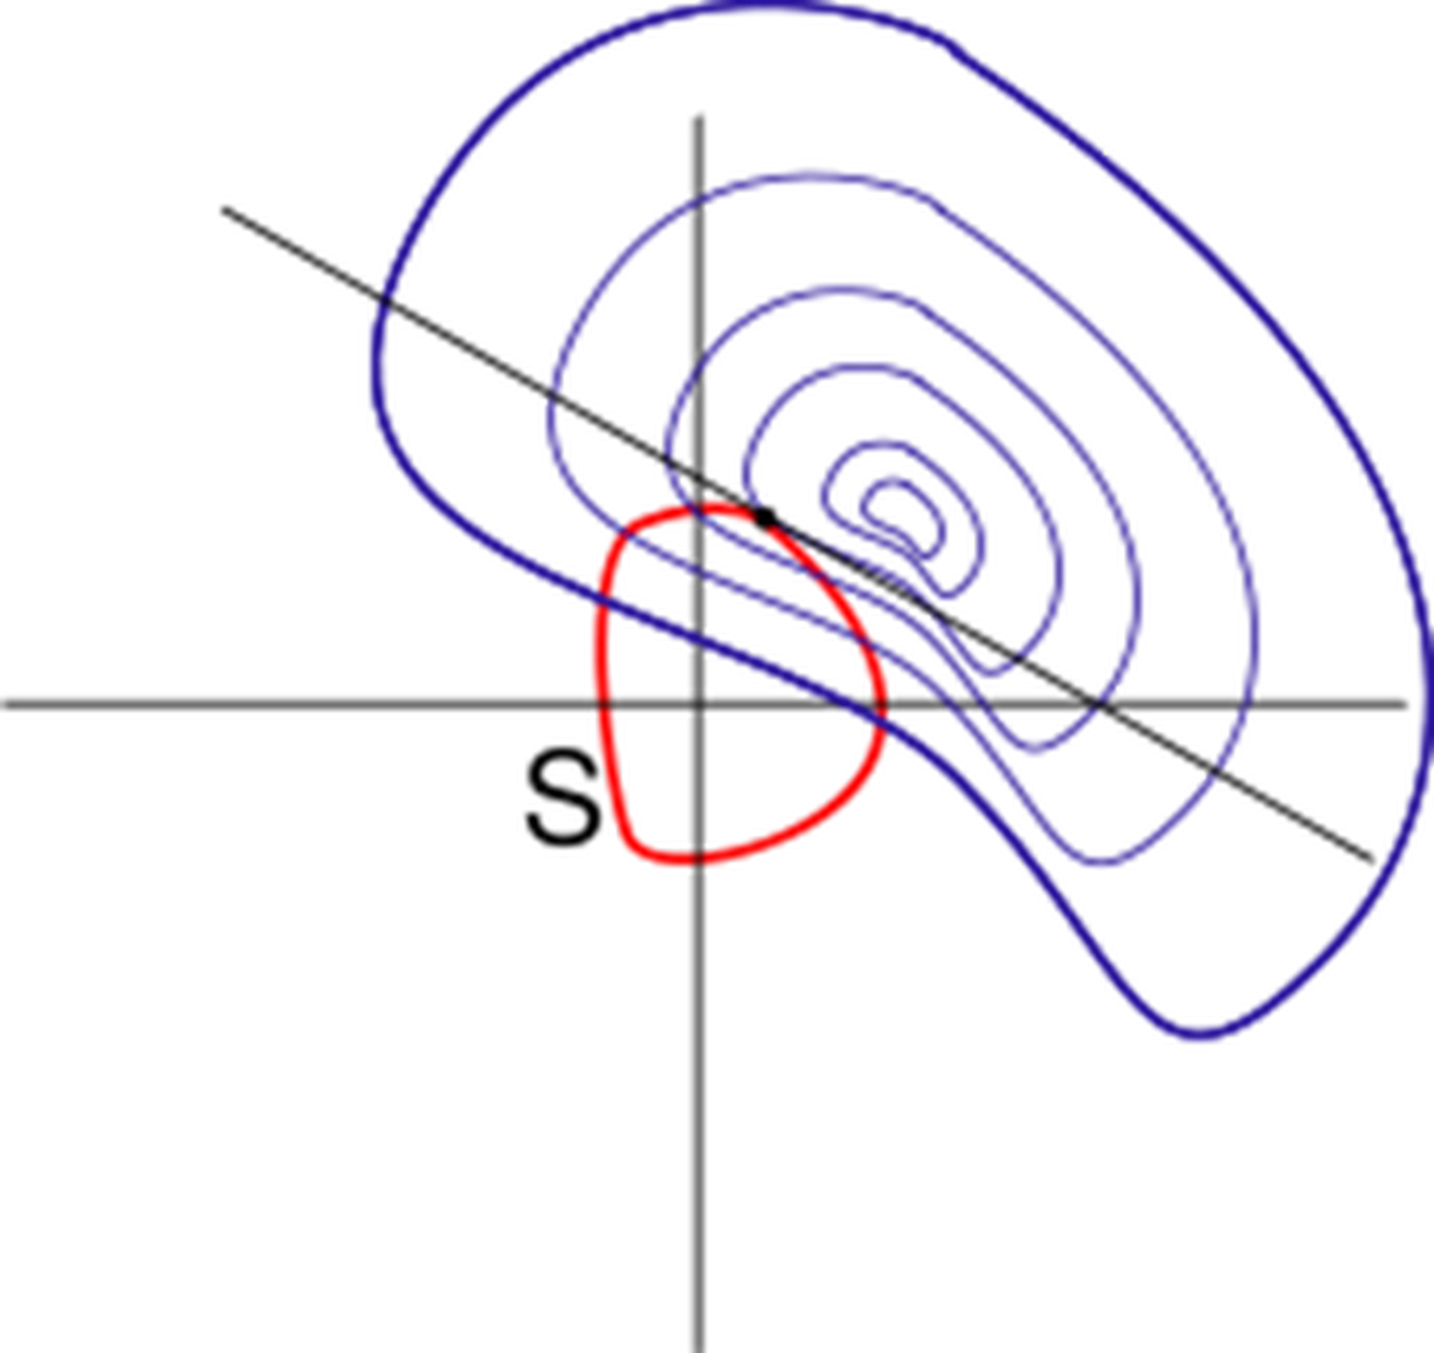
\includegraphics[width=0.5\linewidth]{Additions/pictures/attractor}
\caption{}
\label{}
\end{figure}
%---------------------------------------------------------


\emph{Двовимірний випадок}: Нехай необхідно знайти екстремум деякої функції двох змінних $f(x,y)$ за певної умови, що задається рівнянням $\psi(x,y)=0$. Наприклад: слід знайти максимальну висоту, на яку піднімається група альпіністів по маршруту, заданому кривою $S$: $\psi(x,y)=0$. Нехай функція двох змінних $Z = f(x,y)$ описує форму гори. Тоді криві $Z = \const$ --- криві рівня. Із геометричних міркувань очевидно, що екстремум знаходиться в точці $(x_0, y_0)$, де дотичні до $\psi(x,y)$ та лінії рівня збігаються. Якщо ж маршрут проходить трансвесально під деяким кутом до лінії рівня то, група або іде вниз або вверх. Таким чином, необхідною умовою екстремуму в нашому випадку буде збіг дотичних. Щоб записати його в аналітичній формі, зауважимо, що ця умова еквівалентна умові паралельності градієнтів:

\begin{equation}
	\nabla f|_{x_0,y_0}=\lambda\nabla\psi|_{x_0,y_0}.
	\label{eq:AppA.2}
\end{equation}

Утворимо функцію Лагранжа $L(x,y,\lambda) = f(x,y) - \lambda \psi(x,y,z)$. Необхідною умовою її екстремуму є рівність нулю градієнта $\Delta L(x_0, y_0, \lambda_0) = 0$.
\begin{equation}
\begin{cases}
\dfrac{\partial f(x_0, y_0)}{\partial x} - \lambda \dfrac{\partial \psi(x_0, y_0)}{\partial x} = 0 \\[2ex]
\dfrac{\partial f(x_0, y_0)}{\partial y} - \lambda \dfrac{\partial \psi(x_0, y_0)}{\partial y} = 0 \\[2ex]
\quad \psi(x_0, y_0) = 0
\end{cases}
\end{equation}

Перші два рівняння еквівалентні умові (\ref{eq:AppA.2}), а останнє рівнянню $\psi(x,y)=0$. Із них можна визначити екстремальні значення $x_0, y_0, \lambda_0$.